\documentclass{ctexrep}
\bibliographystyle{plain}
\CTEXsetup[format={\Large\bfseries}]{section}
\usepackage{longtable}
\usepackage{graphicx}
\usepackage{url}
\usepackage{supertabular}
\usepackage{float}
\usepackage{multicol}
\usepackage[a4paper, inner=2.5cm, outer=4cm, top=2cm,bottom=3cm, bindingoffset=1cm]{geometry}
\usepackage{tabularx, makecell, multirow,ulem}
\usepackage{listings,xcolor}
\lstset{
	rulesepcolor= \color{gray}, %代码块边框颜色
	breaklines=true,  %代码过长则换行
	numbers=left, %行号在左侧显示
	numberstyle= \small,%行号字体
	keywordstyle= \color{red},%关键字颜色
	commentstyle=\color{gray}, %注释颜色
	frame=shadowbox%用方框框住代码块
}
\usepackage[bookmarks=true,colorlinks,breaklinks]{hyperref}
\title{\textbf{数据仓库项目报告}}
\author{罗浩1752547,李一珉1752882,张子健1752894}
\date{}
\begin{document}
	\maketitle
	\begin{abstract}
		本报告涉及2019-2020秋季学期数据仓库课程项目的ETL、Instance Matching、数据存储与查询等三个方面。主要介绍了三种(关系型、分布式以及图数据库)存储模型在本项目中的使用情况,它们对应的逻辑与物理模型以及相应的优化和适用范围。
	\end{abstract}
	\tableofcontents
	
	\chapter{数据获取}
	根据课程要求,我们的数据分别来自于 Snap 文本文件以及 Amazon 的网站,下面分别描述针对这两种数据我们的处理方式。
	\section{评论文本文件导入}
	由于文本文件较大,我们采用了自己写的Python脚本来进行导入,操作处理十分简单。建立相应的类,然后从文件中一行一行的读取数据,根据该行冒号之前的内容来判断该行是在处理哪个属性,并对对象的相应属性赋值,最后使用pyodbc将其存入SQL Server\footnote{我们在后续的项目中没有再使用 SQL Server 数据库,将其导入SQL Server 只是作为暂时的存储}数据库中。随本文档附带的脚本文件中包含有本程序,因此不再进行描述。
	\section{网页数据爬取}
	在上一步骤的基础上,我们使用 \begin{lstlisting}[language=sql]
select distinct product_id
from movie_review
	\end{lstlisting}
	就可以获取到所有有待获取信息的电影的ID,将其保存到 csv 文件中,我们就确立了获取数据的目标。为了较为轻松的获取数据,我们使用了最著名的Python网络爬虫库Scrapy(\url{https://scrapy.org/} 来进行爬虫。Scrapy的结构如下图所示。
	\begin{figure}[H]
		\centering
		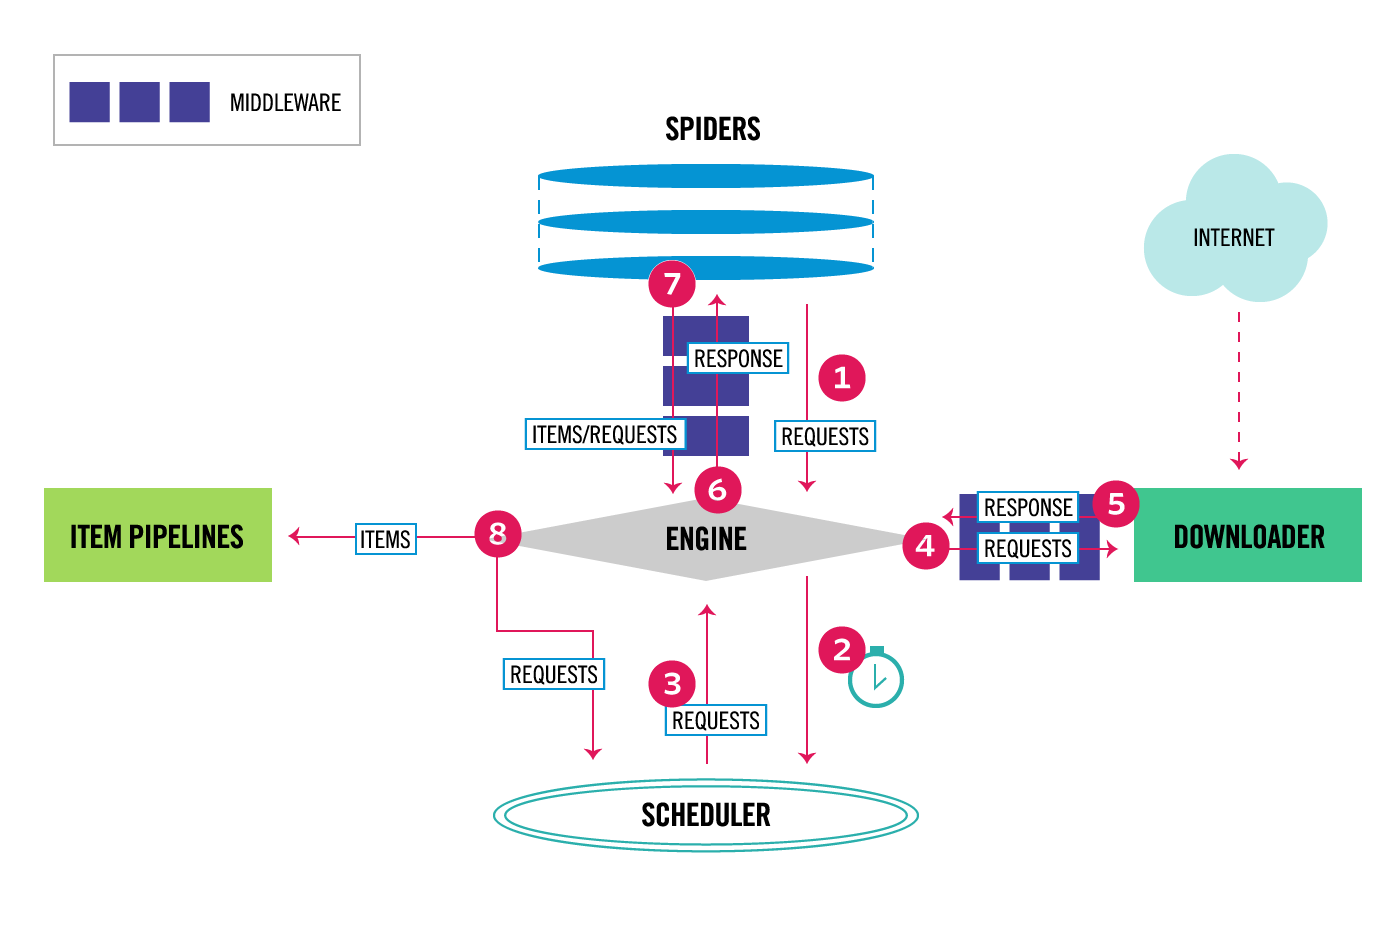
\includegraphics[width=0.7\linewidth]{img/scrapy_architecture_02}
		\caption{Scrapy结构}
		\label{fig:scrapyarchitecture02}
	\end{figure}
	Scrapy能够帮助我们完成发起请求、获取原始HTML文件、将文件递交给Spider进行数据抽取并最终将处理结果传递给流水线进行处理。我们需要主要要写的就是 Spider、PipeLines以及Middleware。下面分别对这三种结构进行描述
	\subsection{Spider}
	Spider 是爬虫的核心,请求的发起以及对HTML文件中数据的抽取都由它来负责。在我们的项目中,请求的发起就是根据上述生成的csv文件来获取完整路径名来进行的。下载的HTML文件会作为参数传递到下述的函数中\begin{lstlisting}[language=python]
 def parse(self, response, **kwargs):
	\end{lstlisting}
	在这个函数中,我们对response做xpath的解析,从而抽取数据。下面给出提取演员时所使用的xpath表达式作为例子\begin{lstlisting}[language=python]
actors = response.xpath(
   '//*[@id="detail-bullets"]/table//tr/td/div/ul/li[{}]/a//text()'.format(i)).extract()
actors = ', '.join(actors)
	\end{lstlisting}
	其他变量的处理也是类似的,不再赘述 \footnote{我们所上交的文件中的xpath现在未必可以正确的提取出数据来,因为Amazon网站有时会修改元素的类名,在类名之前添加随机字符串。例如抽取电影类型的表达式'(//div[@class="\_2vWb4y dv-dp-node-meta-info"]//dl)[1]/dd/a/text()'中的'\_2vWb4y就是我们第二次爬虫的时候修改的(大概在2019年11月),第一次我们爬虫的时候该字段是‘\_3RXp\_N’(大概在2019年国庆节前)。尽管如此,这种处理方式仍是成立的}。
	
	同样值得注意的是,Amazon的电影信息所处在的网页格式并不是唯一的,事实上有两种,分别如下图所示
	\begin{figure}[H]
		\centering
		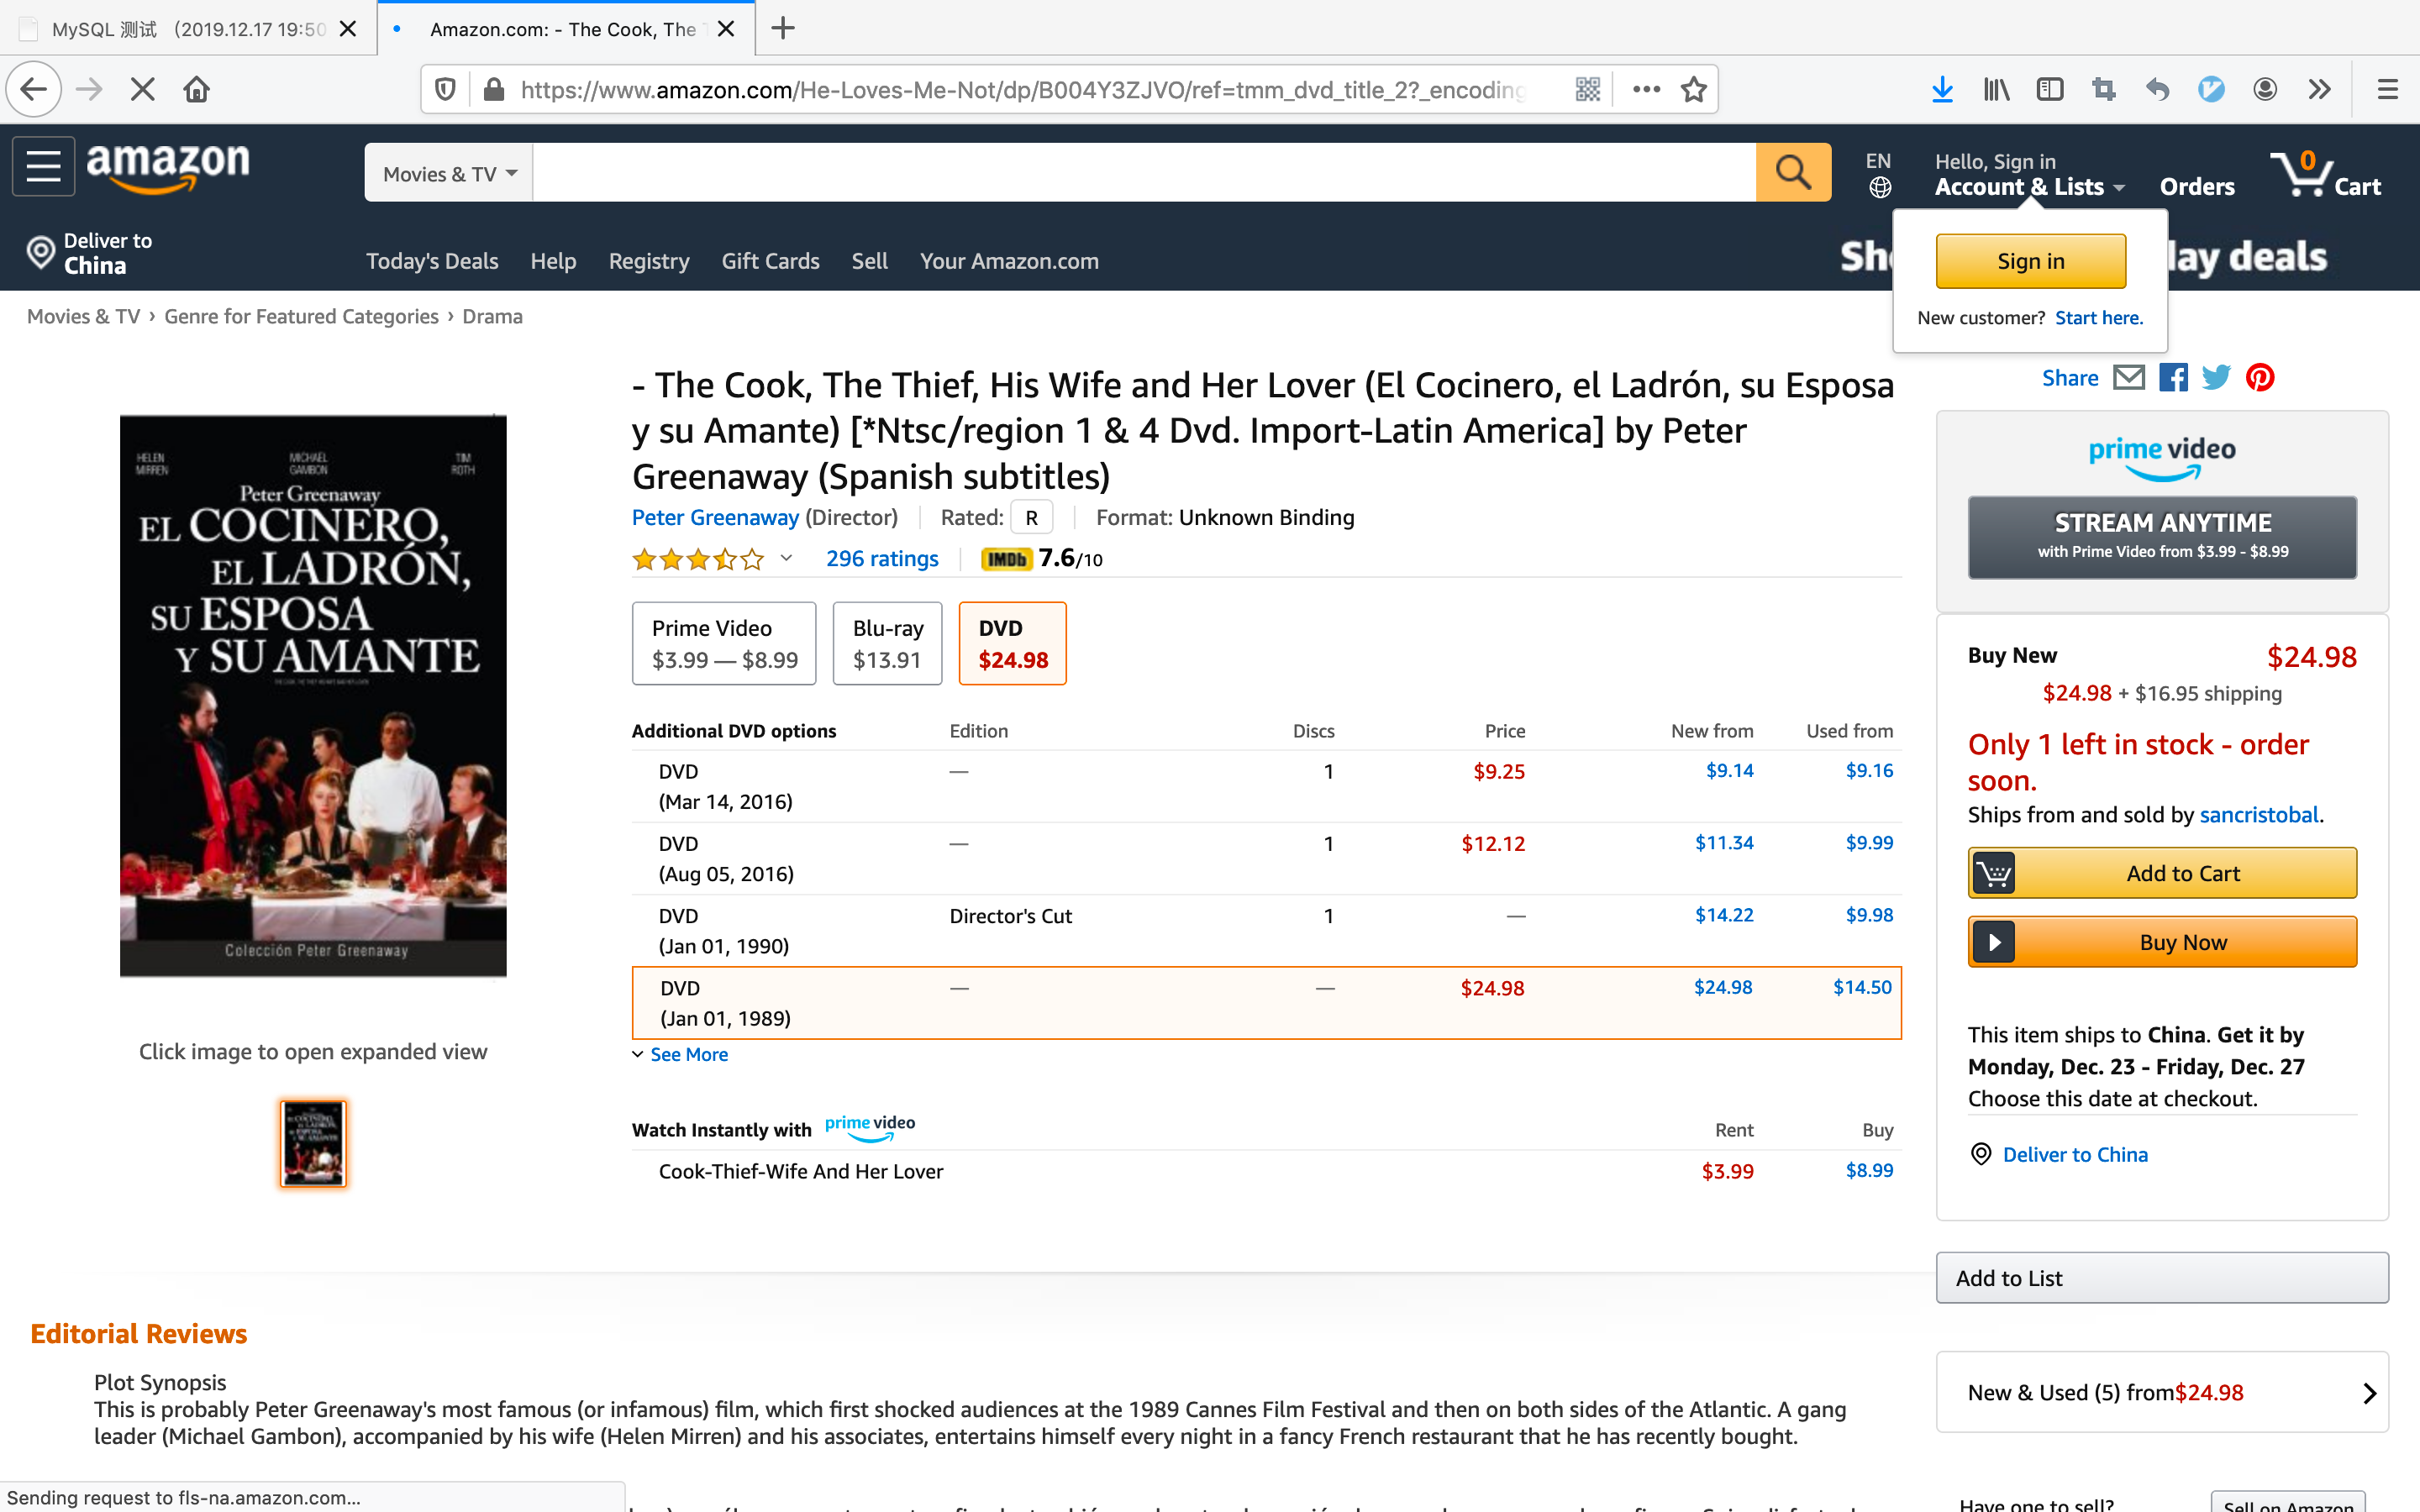
\includegraphics[width=0.7\linewidth]{img/old}
		\caption{老版网页}
		\label{fig:old}
	\end{figure}
	\begin{figure}[H]
		\centering
		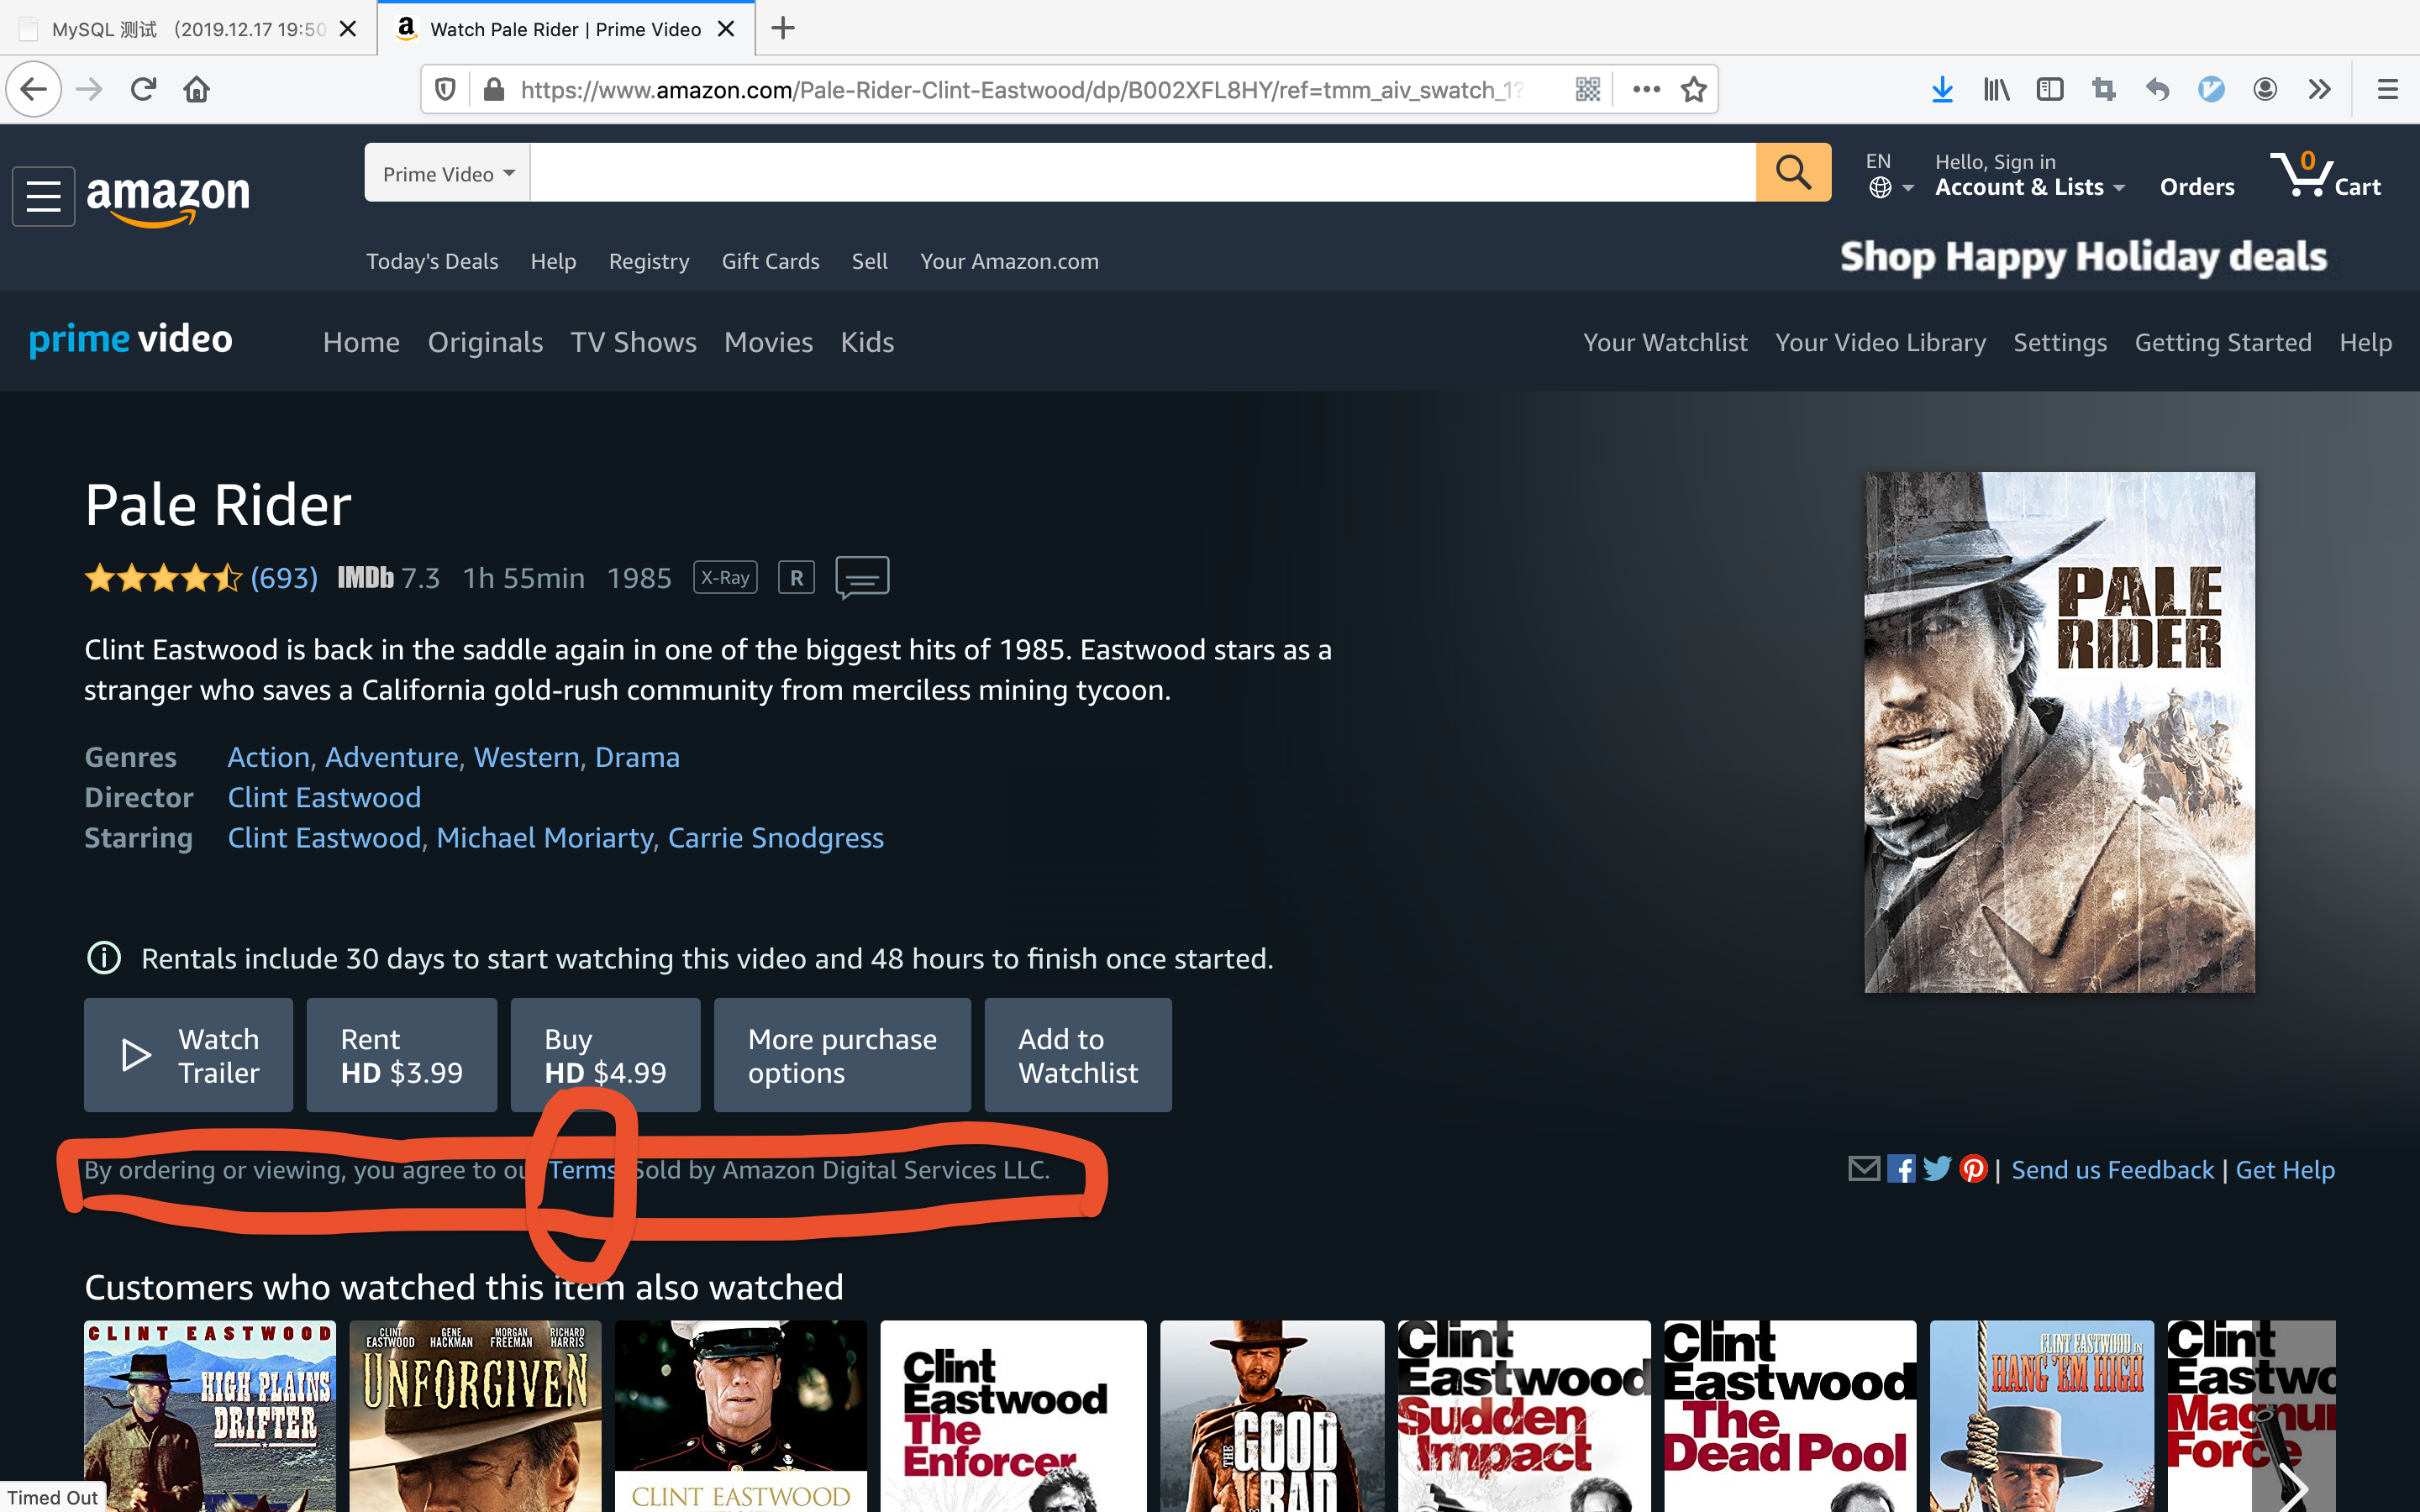
\includegraphics[width=0.7\linewidth]{img/new}
		\caption{新版网页}
		\label{fig:new}
	\end{figure}
	而我们是根据新版网页中的那个 Terms 来进行判断(用红色圈出)的。如果有这个 Terms,我们就会使用针对新版网页写的脚本进行提取,而老版本则使用另外的脚本来提取。
	
	完成相应值的抽取之后,我们将他们都集中到一个对象中,然后使用 yield 将该对象返回,该对象在后面会被送给 Item Pileline 进行处理。大致代码如下:\begin{lstlisting}
oader.add_value('movie_id', movie_id)
loader.add_value('actors', actors)
loader.add_value('directors', directors)
loader.add_value('release_date', release_date)
loader.add_value('movie_type', movie_type)
loader.add_value('movie_version', movie_version)
loader.add_value('movie_title', movie_title)
# print(loader.load_item())
yield loader.load_item()
	\end{lstlisting}
	\subsection{Pipeline}
	在上述的Spider返回对象之后,Pipeline将会收到这些对象,并且在这里对这些对象进行存储或者处理,然后再返回Item对象,以便其他的Pipeline元素处理。在我们的项目中,我们只需要一个pipeline对象来将爬出的数据存储到数据库里就可以了。代码是简明的,大致如下:\begin{lstlisting}
self.cursor.execute("""
  insert into movie_info(movie_id, movie_title, directors, release_date, movie_type, movie_version, actors)
  values (?,?,?,?,?,?,?)
  """, [
    item.get('movie_id')[0], item.get('movie_title')[0], item.get('directors')[0],
    item.get('release_date')[0],
    item.get('movie_type')[0], item.get('movie_version')[0], item.get('actors')[0]
])
self.cnxn.commit()
	\end{lstlisting}
	\subsection{Middleware}
	Middleware主要是在请求发送之前可以对请求的参数进行加工。在我们的项目中,我们主要的需求是设置网络代理。由于需要爬出的电影有25万条,要想在合理的时间之内完成这个项目,爬取的速度必须要快,我们实际使用了百多个线程同时下载。在这种情况下,Amazon将会很快的封锁我们的IP,使得我们无法再继续访问(或者是要求用户来填写一些验证码,需要图像识别)。为了方便起见,我们使用了多贝云动态转发http隧道(\url{http://www.dobel.cn/act/https_pro/index.html}),我们将请求发送给多贝云服务器,然后由它来转发,大致原理如下:\begin{figure}[H]
		\centering
		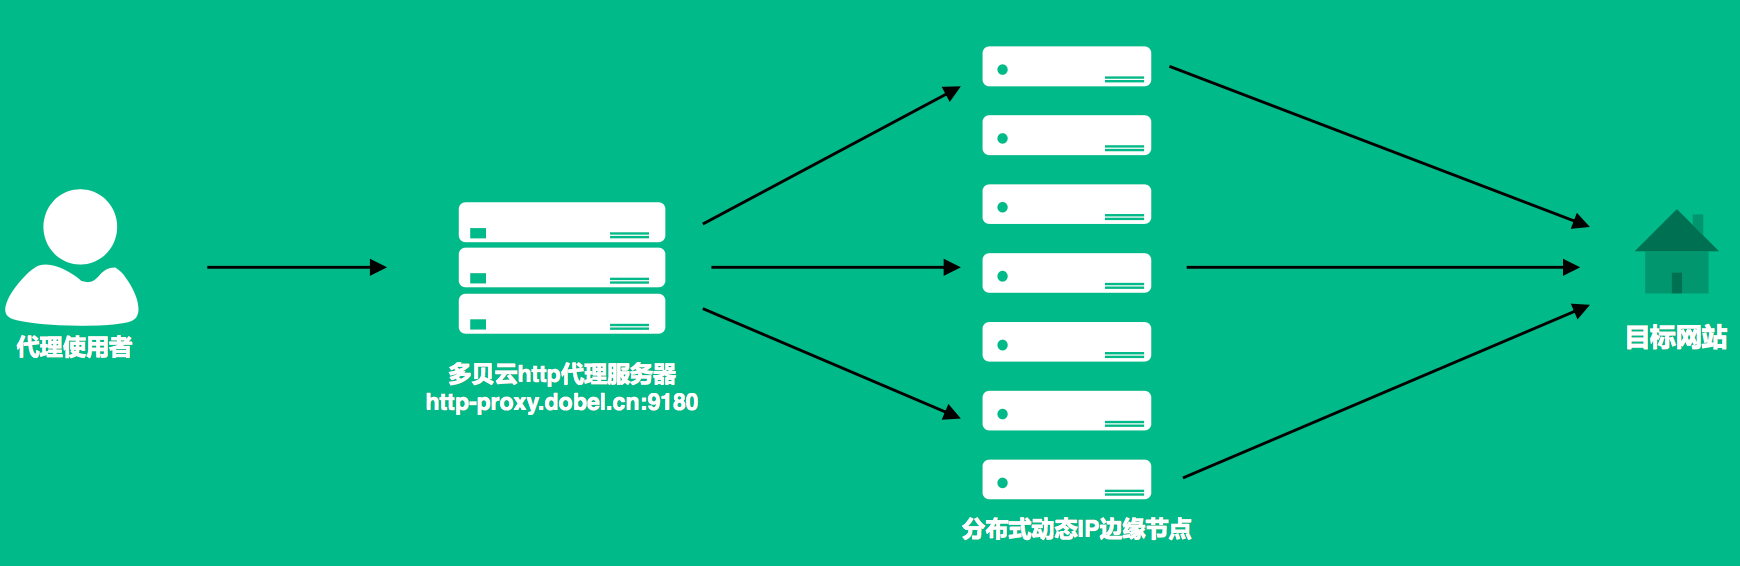
\includegraphics[width=0.7\linewidth]{img/product_desc}
		\caption{多贝云代理}
		\label{fig:productdesc}
	\end{figure}
	
	在具体开始爬虫的时候,我们使用两台电脑共同运行爬虫程序,它们通过上文所述的 pipeline 向同一个数据库中写入爬出的电影数据,从而尽可能的达到最高的请求速度。实际爬虫的速度波动较大,好的时候可以到达100多部电影每分钟,差的时候只有40。下图是我们购买的服务的截图\begin{figure}[H]
		\centering
		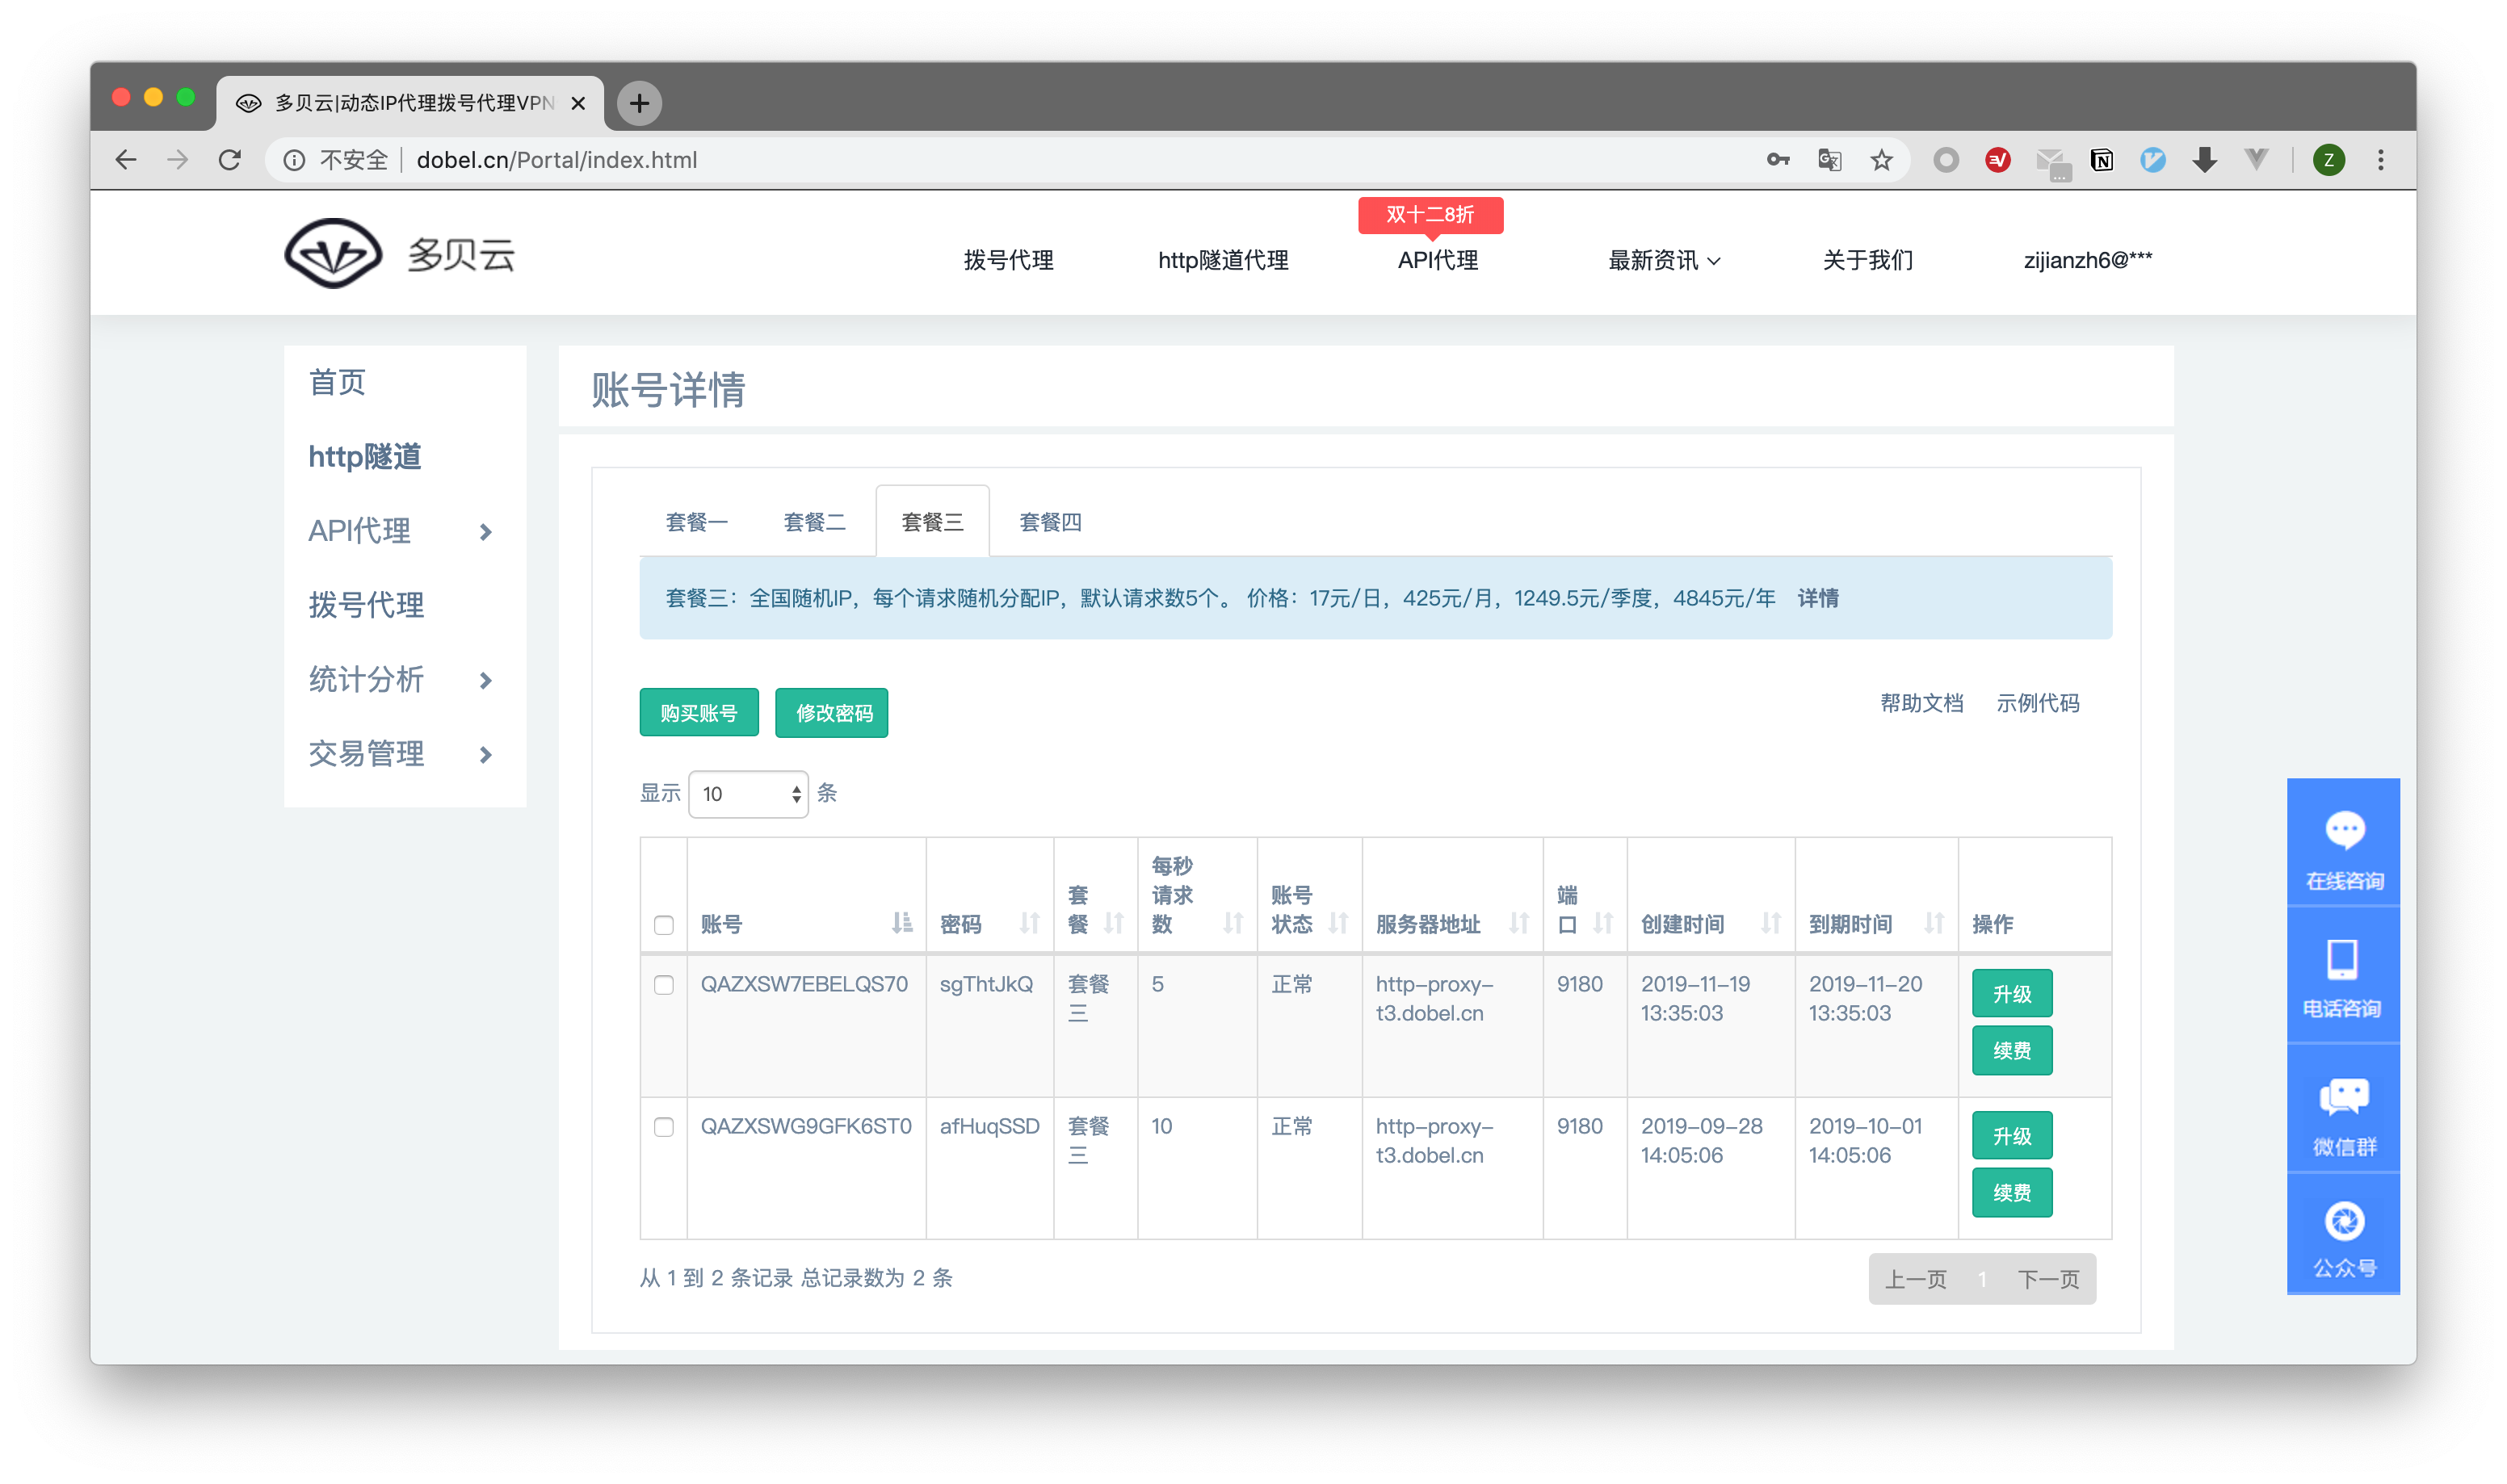
\includegraphics[width=0.7\linewidth]{img/proxy_pay}
		\caption{代理服务}
		\label{fig:proxypay}
	\end{figure}
	可以看到,我们事实上进行了两次爬虫,分别处在刚刚布置这项作业时以及项目正式开始时。第二次其实收获不大,主要是查漏补缺,为数据预处理做好准备。而我们所说的 middle 类正是做这样的代理设置,配置代码如下\begin{lstlisting}[language=python]
def process_request(self, request, spider):
  # 设置代理服务器域名和端口,注意,具体的域名要依据据开通账号时分配的而定
  request.meta['proxy'] = "http-proxy-t3.dobel.cn:9180"
  # 设置账号密码
  proxy_user_pass = "QAZXSW7EBELQS70:sgThtJkQ"
  # setup basic authentication for the proxy
  encoded_user_pass = "Basic " + base64.urlsafe_b64encode(bytes((proxy_user_pass), "ascii")).decode("utf8")
  request.headers['Proxy-Authorization'] = encoded_user_pass
  request.meta['max_retry_times'] = 10
	\end{lstlisting}
	\section{数据获取结果}
	成功获取了所有的评论文本数据以及绝大部分的电影数据。但是由于有的电影链接都已经失效,总共获得了\textbf{252382}行电影信息。
	
	\chapter{数据预处理}
	我们将上一步骤的结果输出为csv文件,就具有了有关电影的信息。为了处理数据中的冗余情况,我们对于数据中的重复项进行了合并,下面分别针对总体结构、判重标准以及合并策略三方面进行描述。
	\section{总体结构}
	由于在课程中朱老师特别强调重视可拓展性多于匹配的准确性,因此我们的处理方式对可拓展性进行了特别的重视,我们采用的是Hadoop的MapReduce模型来进行Instance Matching,以此获得在我们现有知识范围中最佳的可拓展性的同时保持对数据进行较为细粒度处理的可能。大致的处理流程如下图所示\begin{figure}[H]
		\centering
		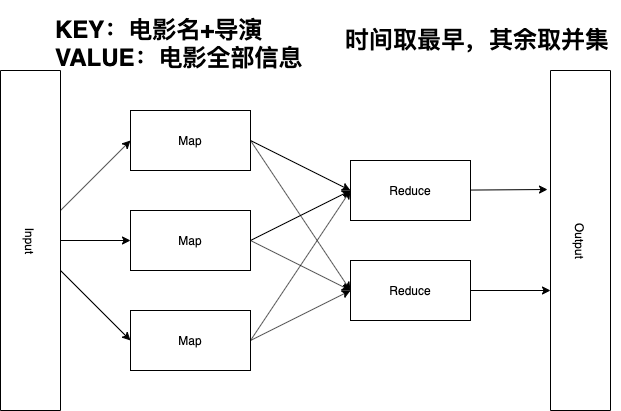
\includegraphics[width=0.7\linewidth]{img/maprecude}
		\caption{Map Reduce示意图}
		\label{fig:maprecude}
	\end{figure}
	
	我们考虑Map Reduce 模型的特征就可以发现如下两个明显特点:\begin{itemize}
		\item Map过程输出的 Key 就代表我们对\textbf{什么是相同电影} 的判断。因为具有相同Key的会被输入同一个Reduce中,这就自动的完成了相同电影的判断。
		\item Reduce 过程对某一个Key下所有Value的处理策略代表我们对\textbf{相同的电影应该怎么合并}的看法。因为它们最终会化为Reduce中的一次输出。
	\end{itemize}
在有了上面两个判断之后,我们再来进行下面的分别对判断标准和合并策略的描述就显得自然了(它们都已经简要的描述在了图 \ref{fig:maprecude} 上)。
	\section{判断标准}
	我们的判断标准非常简单,如果两个电影具有相同的名字和相同的导演(排序之后的导演列表),我们就认为这两个电影是同一部电影。这种判断足够简单,同时也具有一定的效力 \footnote{同一个导演不会拍两个不同的电影还给它们完全相同的名字。}。在这种策略的指导下,我们把思路实现为map函数。由于它还要处理从csv到对象的转化,过程稍显繁杂,下面只摘取最核心的部分进行展示。\begin{lstlisting}[language=java]
// info 是电影对象
List<String> directors = info.getDirector();
// 合并导演
Collections.sort(directors);
StringBuilder directorKey = new StringBuilder();
for (String dire : directors) {
  directorKey.append(dire).append(", ");
}
// lines[1]中是电影名
context.write(new Text(lines[1]+" "+directorKey.toString()), new Text(JSON.toJSONString(info)));
	\end{lstlisting}
	\section{合并策略}
	我们的合并策略也清晰简明。如下表所示\begin{longtable}{l|l}
		\hline
		条目 & 策略 \\
		\hline
		\hline
		时间 & 取最早日期\footnote{后面出来的同一部电影应该是翻拍} \\
		ID、类型、版本、演员 & 取并集\\
		\hline
		\caption{合并策略}
	\end{longtable}
		在这样的策略的指导下,我们可以完成合并,最终我们将电影信息写入Json文件,如下所示\begin{lstlisting}
context.write( NullWritable.get(),new Text(JSON.toJSONString(info)));
\end{lstlisting}
\section{合并结果}
在经过上述的合并之后,电影的数量从\textbf{252382}行下降到\textbf{195891}行,下降了22.3\%.
	
	\chapter{数据存储与查询}
	在完成数据的初步处理之后,我们按照要求将数据分别使用关系型数据库、分布式文件系统以及图数据库进行存储,下面分为三个部分分别对这三种存储方案下的存储模型、优化方案、实验数据以及对改种方案所适合的查询类型的判断的描述。
	\section{关系型数据库}
	\subsection{概述}
	\begin{itemize}
		\item 物理配置是怎么样的?
		\item 整体的想法是怎么样的?
	\end{itemize}
	\subsection{逻辑模型}
	\begin{itemize}
		\item ER图
		\item 必要的说明
	\end{itemize}
	\subsection{物理模型及其优化方案}
	\begin{itemize}
		\item 初步的模型
		\item 改良的模型
		\item \begin{itemize}
			\item 为什么要优化?哪个数据你不满意了?
			\item 怎么优化的?为什么想这样优化?
			\item 优化的结果大概是怎么样的?并且指出在实验数据中的体现
		\end{itemize}
	\end{itemize}
	\subsection{实验数据}
	\subsubsection{按时间查询}
	\begin{itemize}
		\item 样例
		\item 结果
		\item 时间采样(优化前、后)
		\item 平均时间(优化前、后)
	\end{itemize}
	\subsubsection{按电影名称进行查询}
	\subsubsection{按导演进行查询}
	\subsubsection{按演员进行查询}
	\subsubsection{对导演和演员关系进行查询}
	\subsubsection{按电影类别进行查询}
	\subsubsection{按用户评价进行查询}
	\subsubsection{综合查询}
	\subsection{实验结论}
	
	
	\section{分布式文件系统}
	\subsection{概述}
	\subsection{存储模型及其优化方案}
	\subsection{实验数据}
	\subsection{实验结论}
	
	\section{图数据库}
	\subsection{概述}
	根据课程中朱老师的建议,我们使用了最有名的图数据库Neo4j来作为本项目的图数据库部分存储方案。与前两者采用的云端方案不同,我们在图数据库部分直接使用的是Neo4j的桌面版本,以便能够更好的使用Neo4j Browser 来进行数据模型的可视化。总而言之,在图数据库部分选择的软件版本与配置信息如下所示:
	\begin{longtable}{l|l}
		\hline
		条目 & 说明\\
		\hline
		\hline
		Neo4j版本 & 3.5.12 Enterprise\\
		Neo4j Zulu 允许内存 & 6G \\
		\hline
		笔记本操作系统 & Windows 10 专业版 64 位 \\
		笔记本处理器 & Intel(R) Core(TM) i7-7700HQ CPU @ 2.8GHZ \\
		笔记本内存 & 16GB\\
		\hline
		\caption{配置信息}
	\end{longtable}
	在图数据库的存储部分,我们根据项目文档中所提出的常见搜索的要求,将电影以及评论信息分别抽取出相应的节点并且使用边将它们连接起来,主要的节点标签有以下几种:\begin{itemize}
	  	\item MOVIE
	  	\item MOVIE\_ID
	  	\item COMMENT
	  	\item USER
	  	\item ACTOR
	  	\item TYPE
	  	\item DIRECTOR
	  	\item VERSION
	  	\item YEAR
	  	\item QUARTER
	  	\item MONTH
	  	\item DAYOFWEEK
	  	\item DAYOFMONTH
	\end{itemize}
	它们之间具体是怎样连接以及经历了怎样的演化过程,我们将在下一节详细描述。
	\subsection{存储模型及其优化方案}
	在本部分仅仅给出大致时间数据,在下一节中我们给出具体的实验数据。
	\subsubsection{初步模型} \label{neo:1}
	在简单阅读了Neo4j的有关介绍之后,我们快速上手做出了初次原型,使用Neo4j Browser生成的数据库模式图如下所示:
\begin{figure}[H]
	\centering
	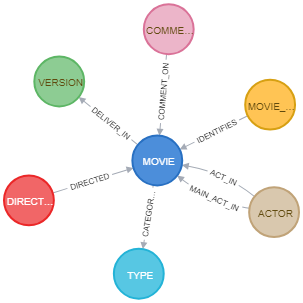
\includegraphics[width=0.7\linewidth]{img/graph1}
	\caption{第一次结构}
	\label{fig:graph1}
\end{figure}
	其中每个标签的节点的具体信息如下表所示\begin{longtable}{l|p{8cm}}
		\hline
		标签 & 属性与索引(加粗字段) \\
		\hline
		\hline
		ACTOR & \textbf{name} \\
		COMMENT & summary, score, review\_time, review\_text, helpfullness, profile\_name, user\_id \\
		DIRECTOR & \textbf{name}\\
		MOVIE & \textbf{name}, score, commentNumber, releaseDate, totalScore \\
		MOVIE\_ID & \textbf{id} \\
		TYPE & \textbf{name}\\
		VERSION & \textbf{name}\\
		\hline
		\caption{节点信息-1}
	\end{longtable}
	我们可以看到,这种建模方式和关系型的建模方式是有类似的地方的。我们将「多值属性」抽离成单独的节点,然后用边(类似于外键)把它们连接起来。事实上这种方式虽然非常简单,但是已经足够可以解决绝大部分的Query了。在向Neo4j数据库插入值的过程中,我们发现随着插入数量的上升,插入的速度会逐渐变慢 \footnote{我们认为因此这个问题的主要原因在于,我们在插入的过程中使用了 MERGE 以及 MATCH 语句,它们事实上涉及到查询,而正是查询消耗了越来越多的时间},为了解决这个问题,我们在插入的过程中建立了以下索引,使得插入速度有了明显的上升,如下图所示,在插入到3万条左右的时候,每插入500条已经需要两份半,在对电影ID加入索引之后时间下降到一分钟,在各个name属性上加入索引之后,插入时间下降到30s左右,并随着插入数量的上升而慢慢上升。
	\begin{figure}[H]
		\centering
		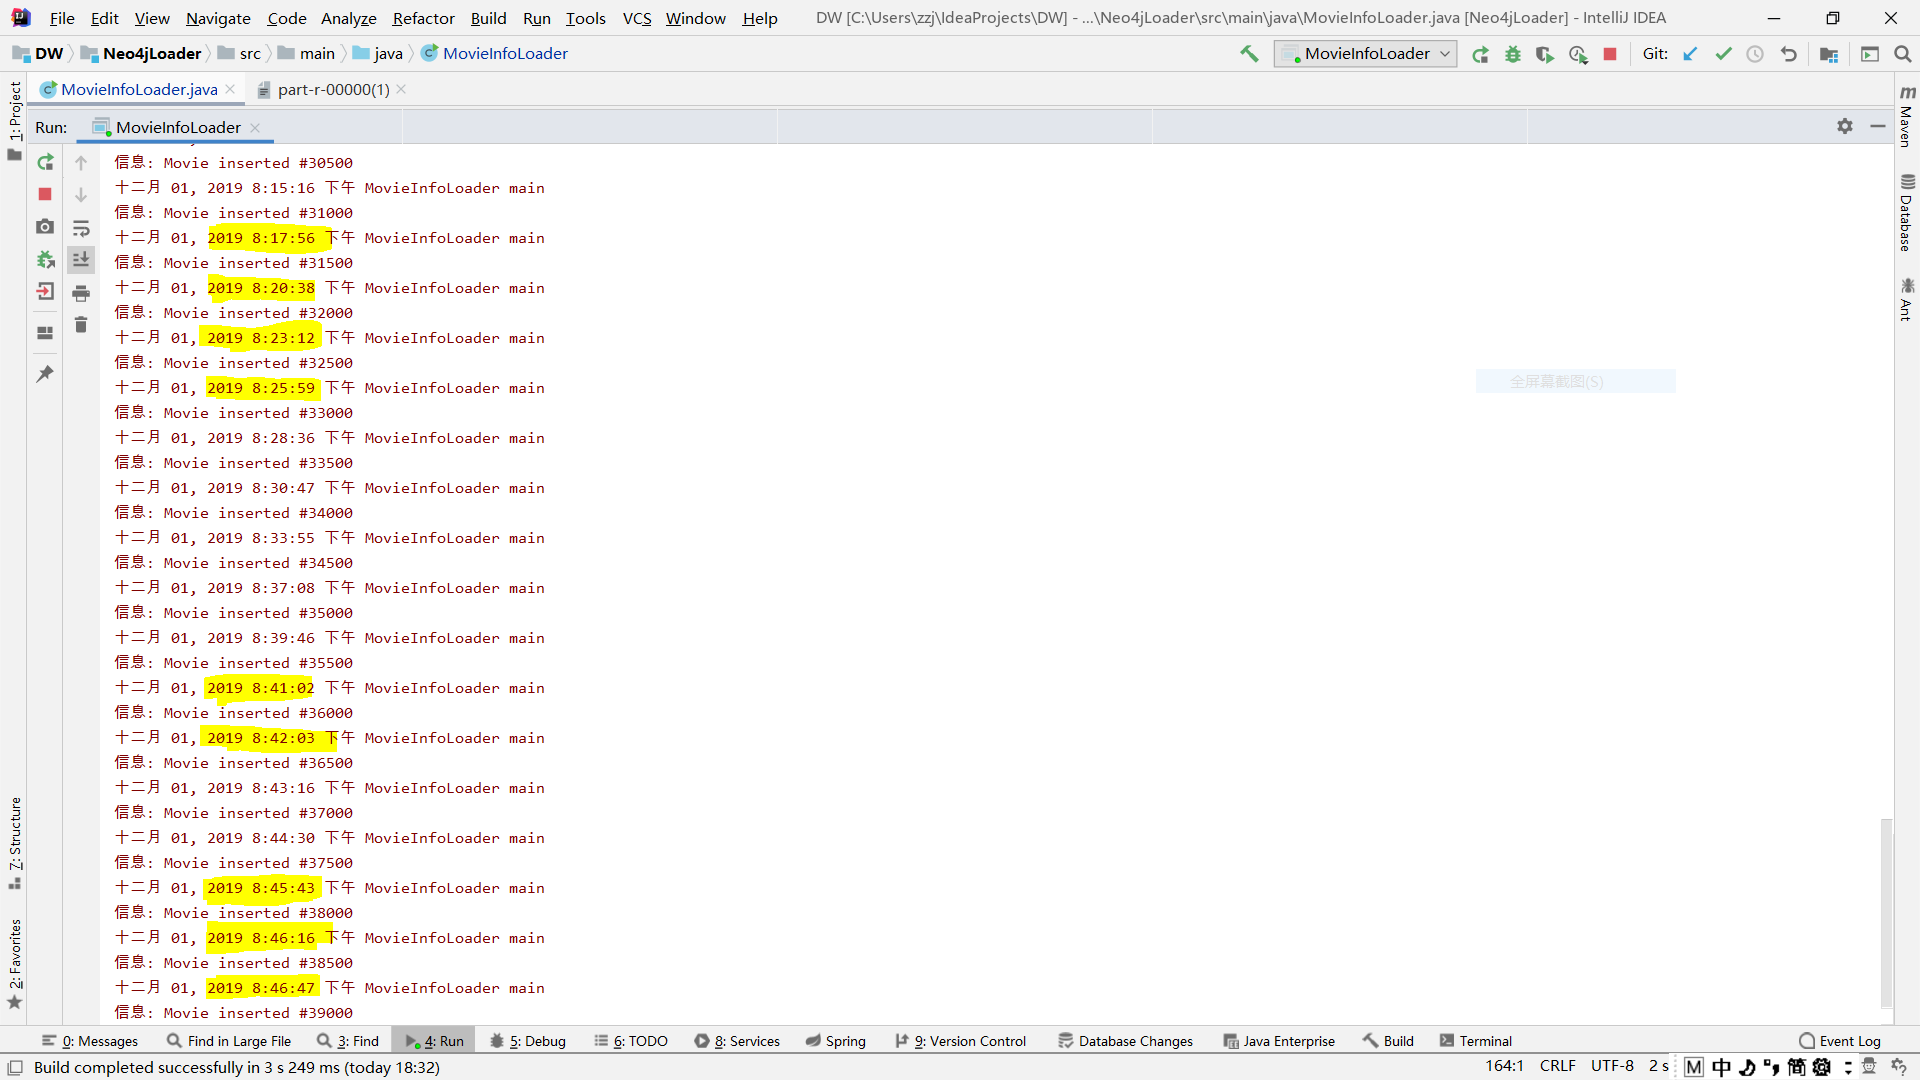
\includegraphics[width=0.7\linewidth]{img/indexInInsersion}
		\caption{插入过程log}
		\label{fig:index}
	\end{figure}
	这种方法存在问题的地方有两个\begin{enumerate}
		\item 时间是使用时间戳来存储的,查询需要自行换算成范围,而对「周二上映的电影有多少」这样的问题实际上无从回答。
		\item 用户没有被显式的抽取,这将给对用户的分析带来不便。
	\end{enumerate}
事实上,后面的各种改动都是针对这样的问题来进行的。
	
	\subsubsection{提取时间} \label{neo:2}
	由于第一种方案中存在的针对时间的查询难以进行的情况,我们提出了新的方案,也即是将时间作为新的节点抽取出来,而不是作为电影节点的属性。同时我们必须考虑到如下问题:\textbf{要怎样构造节点才能使得针对类似于「1998年第一季度所有周二一共有几部电影」这样复合问题的查询变得简明而易于书写?}同时性能上也要有保障。在一番考虑之后,我们采取了如下的节点结构,即使用YEAR、QUARTER、MONTH、DAYOFWEEK以及DAYOFMONTH来构造层次化的结构,使得针对任意组合的查询语句只需要进行拼接就可以完成。具体的结构示意图如下所示:
	\begin{figure}[H]
		\centering
		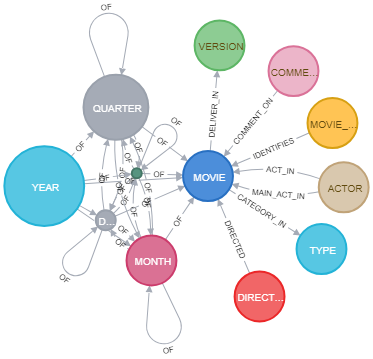
\includegraphics[width=0.7\linewidth]{img/graph2}
		\caption{第二次结构}
		\label{fig:graph2}
	\end{figure}
	
	其中每个标签的节点的具体信息如下表所示\begin{longtable}{l|p{8cm}}
		\hline
		标签 & 属性与索引(加粗字段)  \\
		\hline
		\hline
		YEAR & num\\
		QUARTER & num \\
		MONTH & num\\
		DAY\_OF\_MONTH & num\\
		DAY\_OF\_WEEK & num \\
		\hline
		ACTOR & \textbf{name} \\
		COMMENT & summary, score, review\_time, review\_text, helpfullness, profile\_name, user\_id \\
		DIRECTOR & \textbf{name}\\
		MOVIE & \textbf{name}, \textbf{score}, commentNumber, releaseDate, totalScore \\
		MOVIE\_ID & \textbf{id} \\
		TYPE & \textbf{name}\\
		VERSION & \textbf{name}\\
		\hline
		\caption{节点信息-2}
		\end{longtable}
	在采取了这样的方式之后,由于每个时间节点之间都是OF关系,我们的查询语句的拼接变得非常简单,使用如下所示的结构可以轻松的完成针对任意组合条件进行的查询。\begin{lstlisting}[language=java]
if(timeFrom.getYear() != 0){
  matchingClause += "(y:YEAR{num: " + timeFrom.getYear() +" })-[:OF]->";
}
if(timeFrom.getQuarter() != 0){
  matchingClause += "(q:QUARTER{num: "+ timeFrom.getQuarter() +" })-[:OF]->";
}
if(timeFrom.getMonth() != 0){
  matchingClause +="(m:MONTH{num: "+ timeFrom.getMonth() +" })-[:OF]->";
}
if(timeFrom.getDay_of_week() != 0){
  matchingClause +="(dow:DAY_OF_WEEK{num: "+ timeFrom.getDay_of_week() +" })-[:OF]->";
}
if(timeFrom.getDay_of_month() != 0){
  matchingClause +="(dom:DAY_OF_MONTH{num: "+ timeFrom.getDay_of_month() +"})-[:OF]->";
}
	\end{lstlisting}
	
	\subsubsection{提取用户}\label{neo:3}
	为了分析与用户有关的数据,我们必须把原本的评论节点中的有关用户的信息进行抽取,使它们成为单独的节点,从而便于后续的处理。因此,我们对原来的结构进行了拓展,使得结构整体如下图所示:
	\begin{figure}[H]
		\centering
		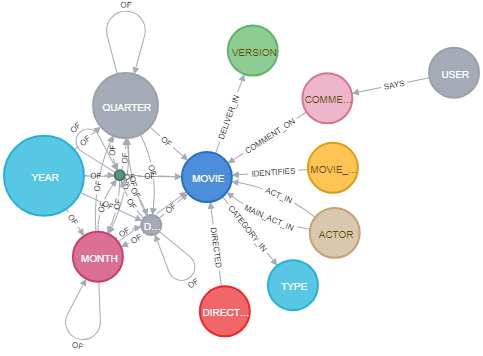
\includegraphics[width=0.7\linewidth]{img/graph3}
		\caption{第三次结构}
		\label{fig:graph3}
	\end{figure}
	
	其中每个标签的节点的具体信息如下表所示\begin{longtable}{l|p{8cm}}
		\hline
		标签 & 属性与索引(加粗字段)  \\
		\hline
		\hline
		USER & \textbf{profile\_name}, \textbf{user\_id }\\
		\hline
		YEAR & num\\
		QUARTER & num \\
		MONTH & num\\
		DAY\_OF\_MONTH & num\\
		DAY\_OF\_WEEK & num \\
		ACTOR & \textbf{name} \\
		COMMENT & summary, score, review\_time, review\_text, helpfullness, profile\_name, user\_id \\
		DIRECTOR & \textbf{name}\\
		MOVIE & \textbf{name}, \textbf{score}, commentNumber, releaseDate, totalScore \\
		MOVIE\_ID & \textbf{id} \\
		TYPE & \textbf{name}\\
		VERSION & \textbf{name}\\
		\hline
		\caption{节点信息-3}
	\end{longtable}
	在进行了这样的修改之后,类似于「某某用户喜欢的电影有哪些?」这样的查询已经可以相对快速的进行了,但是我们希望可以再进一步,完成这样的一组查询\textbf{哪些用户是相似的?}这样的查询所具有的意义是非凡的。我们首先定义什么是相似的:如果两个用户在对同一部电影的评分上相差无几,我们就认为这两位用户对该电影的看法是一致的,如果两个用户在相当数目的电影上的看法都是一致的,我们就可以认为两个用户对于电影的爱好是一致的。如果两个用户被判断为一致的,那么我们就可以将一个用户喜欢而另一个用户还没有看过的电影推荐给还没有看过的那位用户,这部电影会有较大的概率被这个用户喜欢。因此我们尝试在现有的结构上进行这样的查询:\begin{lstlisting}
match (u1:USER)-[:SAYS]->(c1:COMMENT)-[:COMMENT_ON]->(m:MOVIE)<-[:COMMENT_ON]-(c2:COMMENT)<-[:SAYS]-(u2:USER) where abs(c1.score-c2.score)<=1 return u1,u2,count(m) order by count(m) desc
	\end{lstlisting}
	但是经过我们的实验发现,这样的查询在我们现有的6G内存上是远远无法完成的,Neo4j会报告内存溢出并停止查询。在这种情况下我们咨询了朱老师,朱老师建议我们限制查询的电影和评论数量,只考虑最火的那些电影,并对它们进行处理。结合朱老师的建议,我们再对图的结构进行了一次改进,从而可以在较大的粒度上实现这个功能。具体的优化方式如下一节所提到的。
	\subsubsection{优化用户聚类} \label{neo:4}
	由于现在用户连接到自己所评论的电影中间需要经过大量的评论节点,我们猜测这有可能会导致对于内存的大量使用,因此我们将用户和电影之间直接连接起来,从而节省内存的使用。为了进一步简化数据库所必须要做出的操作,我们甚至在数据库内部做出了这样的规定:所有评分高于4分的被认为是喜欢,从而直接使用LIKES边进行连接。这使得二者之间的连接关系进一步的简化。但是仅仅做出这样的改变是不够的,我们还需要像朱老师提到的那样限制电影的数量来使得查询在合适的时间范围内进行。在我们现在的设备上,我们只能考虑评论数量在700以上的电影。至此,我们相当于在受限的条件上完成了我们想进行的搜索,而上文中关于相似的定义事实上在这里被窄化到:如果两个用户都喜欢一部电影,那么这两个用户被在这部电影上的看法被认为是类似的。同样,在此时我们的存储整体结构如下图所示:
	\begin{figure}[H]
		\centering
		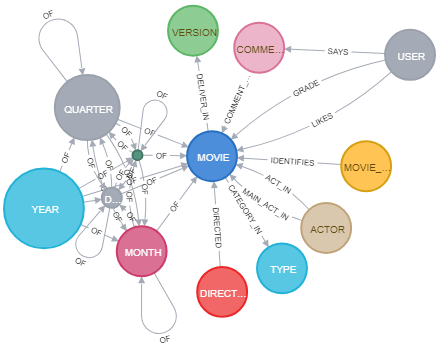
\includegraphics[width=0.7\linewidth]{img/graph4}
		\caption{第四次结构}
		\label{fig:graph4}
	\end{figure}
	其中每个标签的节点的具体信息如下表所示\begin{longtable}{l|p{8cm}}
		\hline
		标签 & 属性与索引 (加粗字段) \\
		\hline
		\hline
		USER &\textbf{ profile\_name}, \textbf{user\_id} \\
		YEAR & num\\
		QUARTER & num \\
		MONTH & num\\
		DAY\_OF\_MONTH & num\\
		DAY\_OF\_WEEK & num \\
		ACTOR & \textbf{name} \\
		COMMENT & summary, score, review\_time, review\_text, helpfullness, profile\_name, user\_id \\
		DIRECTOR & name\\
		MOVIE & \textbf{name}, \textbf{score}, \textbf{commentNumber}, releaseDate, totalScore \\
		MOVIE\_ID & \textbf{id} \\
		TYPE & \textbf{name}\\
		VERSION & \textbf{name}\\
		\hline
		\caption{节点信息-4}
	\end{longtable}
	\subsection{实验数据}
	\subsubsection{按时间查询}
	\begin{enumerate}
		\item 某某年上映了多少电影?\begin{itemize}
			\item 样例:2008 年上映了多少电影?
			\item 结果:11593
			\item 平均执行时间:20-30ms。本查询在 \ref{neo:2} 方案中才能实现,在之后没有明显变化。
		\end{itemize}
		\item 某某年某某月上映了多少电影?\begin{itemize}
			\item 样例:2008 年 1 月上映多少电影?
			\item 结果:2162
			\item 平均执行时间:20ms。本查询在 \ref{neo:2} 方案中才能实现,在之后没有明显变化。
		\end{itemize}
		\item 某某年某某季度上映了多少电影?\begin{itemize}
			\item 样例:2008 年第一季度上映了多少电影?
			\item 结果:3699
			\item 平均执行时间:40ms。本查询在 \ref{neo:2} 方案中才能实现,在之后没有明显变化。
		\end{itemize}
		\item 周某上映多少电影?\begin{itemize}
			\item 样例:周二上映多少电影?
			\item 结果:35619
			\item 平均执行时间:32ms。本查询在 \ref{neo:2} 方案中才能实现,在之后没有明显变化。
		\end{itemize}
	\end{enumerate}
	\subsubsection{按电影名称进行查询}
	 说明:在我们的项目中,为了降低用户搜索难度,使用的是模糊搜索,这导致对于电影名的搜索非常缓慢而几乎不能完成。下面的数据来自于非模糊搜索的结果。
		\begin{enumerate}
		\item 某某电影共有哪些版本?\begin{itemize}
			\item 样例:电影”Beat Street"共有哪些版本?
			\item 结果:\begin{lstlisting}
"data": [
  "Prime Video (streaming online video)",    
 "Prime Video",
 "Blu-ray",
 "DVD"
],
			\end{lstlisting}
			\item 平均执行时间:50ms。本查询在方案 \ref{neo:1}中就可以实现,并且之后没有明显变化。
		\end{itemize}
		\item 某某电影是什么类型的?\begin{itemize}
			\item 样例:电影“Beat Street”是什么类型的?
			\item 结果:\begin{lstlisting}
"data": [
  "Drama",
  "Music Videos and Concerts",
  "All MGM Titles",
  "Musicals"
]
			\end{lstlisting}
			\item 平均执行时间:1ms\footnote{不知道为何会有这样的速度,我们猜测是缓存}。本查询在方案 \ref{neo:1}中就可以实现,并且之后没有明显变化。
		\end{itemize}
		\item 某某电影在什么时候上映?\begin{itemize}
			\item 样例:电影"Beat Street"在什么时候上映?
			\item 结果:\begin{lstlisting}
"data": [
  "1984-1-1",
  "2003-4-15"
]
			\end{lstlisting}
			\item 平均执行时间:10ms\footnote{波动巨大,有时0ms}。本查询在方案 \ref{neo:1}中就可以实现,并且之后没有明显变化。
		\end{itemize}
		\item 某某电影有多少同名电影?\begin{itemize}
			\item 样例:电影“Beat Street”有多少同名电影?
			\item 结果:4
			\item 平均执行时间:295ms。本查询在方案 \ref{neo:1}中就可以实现,并且之后没有明显变化。
		\end{itemize}
		\item 某某电影有哪些演员?\begin{itemize}
			\item 样例:电影“Beat Street”有哪些演员参演?
			\item 结果:\begin{lstlisting}
"data": [
  "Jon Chardiet",
  "Saundra Santiago",
  "Guy Davis",
  "Leon W. Grant",
  "Rae Dawn Chong"
]
			\end{lstlisting}
			\item 平均执行时间:150ms。 本查询在方案 \ref{neo:1}中就可以实现,并且之后没有明显变化。
		\end{itemize}
		\item 某某电影导演是谁?\begin{itemize}
			\item 样例:电影”Beat Street“导演是谁?
			\item 结果:Stan Lathan
			\item 平均执行时间:50ms。\footnote{波动巨大,有时0ms}本查询在方案 \ref{neo:1}中就可以实现,并且之后没有明显变化。
		\end{itemize}
		\item 某某电影有哪些评论?\begin{itemize}
			\item 样例:电影”Beat Street“有哪些评论?
			\item 结果:\begin{lstlisting}
""This ain't New York, this is the Bronx!""
"Yay Breakin!"
"Old School At It's Best"
"A MUST HAVE !!!!!"
"Great Film"
"Love this Movie and Soundtracks"
...
			\end{lstlisting}
			\item 平均执行时间:5ms。\footnote{波动巨大,有时0ms}本查询在方案 \ref{neo:1}中就可以实现,并且之后没有明显变化。
		\end{itemize}
	\end{enumerate}
	\subsubsection{按导演进行查询}
		\begin{enumerate}
		\item 某某导演执导了哪些电影?\begin{itemize}
			\item 样例:Yossi Wein 执导了哪些电影?
			\item 结果:\begin{lstlisting}
"Operation Delta Force 5: Random Fire",
"Fugitive Rage / Merchant Of Death",
"Death Train",
"Octopus 2:River of Fear VHS",
"U.S. Seals",
"U.S. Seals - Dead Or Alive VHS",
"Us Seals",
"Disaster",
"Merchant of Death",
"Octopus 2: River of Fear",
"Death Train VHS",
"Cult of Fury",
"Operation Delta Force V:Random Fire VHS",
"Never Say Die VHS"
			\end{lstlisting}
			\item 平均执行时间:50ms\footnote{时间波动极大,有时只要几毫秒}。本查询在方案 \ref{neo:1}中就可以实现,并且之后没有明显变化。
		\end{itemize}
	\end{enumerate}
	\subsubsection{按演员进行查询}
		\begin{enumerate}
		\item 某某演员在哪些电影中担任主演?\begin{itemize}
			\item 样例:Harry Shannon 在那些电影中担任主演?
			\item 结果:\begin{lstlisting}
"Yellow Rose of Texas VHS",
"Kansas Pacific",
"Song Of Texas VHS",
"Kansas Pacific VHS",
"The Yellow Rose of Texas",
"Song of Texas VHS",
"I Love Lucy: Season 1, Vol.3",
"The Yellow Rose of Texas VHS"
			\end{lstlisting}
			\item 平均执行时间:60ms。\footnote{时间波动极大,有时只要几毫秒}本查询在方案 \ref{neo:1}中就可以实现,并且之后没有明显变化。
		\end{itemize}
		\item 某某演员参演多少电影?\begin{itemize}
			\item 样例:Harry Shannon 在那些电影中参演过?
			\item 结果:\begin{lstlisting}
"Yellow Rose of Texas VHS",
"The Yellow Rose of Texas VHS",
"The Yellow Rose of Texas",
"Song of Texas VHS",
"Song Of Texas VHS",
"Song of Texas",
"Kansas Pacific",
"Kansas Pacific VHS",
"Cow Town",
"I Love Lucy: Season 1, Vol.3"
			\end{lstlisting}
			\item 平均执行时间:35ms。本查询在方案 \ref{neo:1}中就可以实现,并且之后没有明显变化。
		\end{itemize}
	\end{enumerate}
	\subsubsection{对导演和演员关系进行查询}
		\begin{enumerate}
		\item 经常合作的演员有哪些?\begin{itemize}
			\item 样例:经常合作的演员有哪些?
			\item 结果:使用32作为门槛。\begin{lstlisting}
"Claudia Black & Ben Browder for 66time(s)",
"Terry Gilliam & Graham Chapman for 62time(s)",
"Tom Baker & Patrick Troughton for 108time(s)",
"Noel MacNeal & Tyler Bunch for 55time(s)",
"Alexandra Isles & Joan Bennett for 38time(s)",
"Trigger & Roy Rogers for 88time(s)",
"Courteney Cox & Jennifer Aniston for 56time(s)",
...
			\end{lstlisting}
			\item 平均执行时间:5500-8000ms本查询在方案 \ref{neo:1}中就可以实现,并且之后没有明显变化。
		\end{itemize}
		\item 经常合作的演员和导演有哪些?\begin{itemize}
			\item 样例:经常合作的导演有哪些?
			\item 结果:使用32作为门槛。\begin{lstlisting}
"Basil Rathbone & Roy William Neill for 79time(s)",
"Megumi Hayashibara & Takeshi Mori for 65time(s)",
"Robert Smigel & Robert Smigel for 37time(s)",
"Richard Ian Cox & Naoya Aoki for 39time(s)",
"Tim Russ & Kenneth Biller for 39time(s)", 
"Peter Linz & Jim Martin for 48time(s)",
"Claudia Black & Ian Watson for 48time(s)",
"Lynne Thigpen & Jim Martin for 41time(s)",
"Kappei Yamaguchi & Tomomi Mochizuki for 54time(s)",
"Justin Cook & Noriyuki Abe for 43time(s)",
"Marc Weiner & Sherie Pollack for 43time(s)",
"n & a for 193time(s)",
"Anthony Simcoe & Geoff Bennett for 48time(s)",
"n & n for 193time(s)",
"Trigger & William Witney for 57time(s)",
"Roy Rogers & William Witney for 69time(s)",
"Charles Chaplin & Charles Chaplin for 54time(s)",
"Jonathan Hardy & Ian Watson for 43time(s)",
"Laura Bailey (II) & Noriyuki Abe for 43time(s)",
"Charles Hawtrey & Gerald Thomas for 62time(s)",
"John Wayne & John Ford for 59time(s)",
...
			\end{lstlisting}
			\item 平均执行时间:1427ms。本查询在方案 \ref{neo:1}中就可以实现,并且之后没有明显变化。
		\end{itemize}
		\item 经常合作的导演有哪些?\begin{itemize}
			\item 样例:经常合作的导员和演员有哪些?
			\item 结果:使用32作为门槛。\begin{lstlisting}
"Cliff Bole & Gabrielle Beaumont for 167time(s)",
“Ikur? Sat? & Hirokazu Yamada for 33time(s)",
"Geoff Bennett & Ian Watson for 48time(s)",
"Gary Goldman & Don Bluth for 38time(s)",
"N & A for 36time(s)",
"Gates McFadden & LeVar Burton for 128time(s)",
"Rocky Collins & Matthew Collins (III) for 53time(s)",
"Robert Becker & LeVar Burton for 128time(s)",
"Angela Santomero & John Rowe for 33time(s)",
 "Arthur Rankin Jr. & Jules Bass for 68time(s)",
"LeVar Burton & Cliff Bole for 128time(s)",
...
			\end{lstlisting}
			\item 平均执行时间:897ms。本查询在方案 \ref{neo:1}中就可以实现,并且之后没有明显变化。
		\end{itemize}
	\end{enumerate}
	\subsubsection{按电影类别进行查询}
		\begin{enumerate}
		\item 某某类型的电影有多少?\begin{itemize}
			\item 样例:类型为 Action的电影有多少?
			\item 结果:23055
			\item 平均执行时间:本查询在方案 \ref{neo:1}中就可以实现,并且之后没有明显变化。
		\end{itemize}
	\end{enumerate}
	\subsubsection{按用户评价进行查询}
		\begin{enumerate}
		\item 评分为某某的电影有哪些?\begin{itemize}
			\item 样例:观众平均评分为 5 的电影有哪些?
			\item 结果:\begin{lstlisting}
"Andy's Airplanes, Andy Meets the Blue Angels",
"Animal Rescue, Vol. 2: Best Cat Rescues",
"Animals Rock with Lucas Miller! Vol. 1 Monarchs, Metamorphosis and More!",
"Animals and Man Animal Safari, vol.6  VHS",
"Animals of the Amazon Animal Safari, vol.2  VHS",
"Animals of the Rain Forest Art Lessons for Children, Vol. 5  VHS",
"Animaniacs, Vol. 4",
"Animorphs - The Invasion Series, Part 2: Nowhere to Run VHS",
...
			\end{lstlisting}
			\item 平均执行时间:75ms。本查询在方案 \ref{neo:3}中就可以实现,并且之后没有明显变化。
		\end{itemize}
		\item 某某用户喜欢的电影有哪些?\begin{itemize}
			\item 样例:用户ID为AWKP2OZY4WB8M的用户喜欢(评分大于4)的电影有哪些?
			\item 结果:\begin{lstlisting}
"Vampire Princess Miyu: The Last Shinma - Volume 6"
"Vampire Hunter D: Bloodlust"
"Vampire Hunter D"
"Vampire Hunter D VHS"
"Vampire Hunter D - Bloodlust VHS"
"Vampire Hunter D - Bloodlust"
"Spirited Away"
			\end{lstlisting}
			\item 平均执行时间:600ms\footnote{受缓存影响极大}。本查询在方案 \ref{neo:3}中就可以实现,并且之后没有明显变化。
		\end{itemize}
	\end{enumerate}
	\subsubsection{综合查询}
		\begin{enumerate}
		\item 相似的用户有哪些?\begin{itemize}
			\item 样例:相似的用户有哪些?
			\item 结果:\begin{lstlisting}
Lawrance M. Bernabo & Jenny J.J.I. "A New Yorker" 51times
Monkdude & Wayne Klein "If at first the idea is not absu... 47times
...
			\end{lstlisting}
			\item 平均执行时间:110531ms。本查询在方案 \ref{neo:4}中就可以实现,并且之后没有明显变化。
		\end{itemize}
	\end{enumerate}
	\subsection{实验结论}
	综合以上的探索,我们可以得到以下的结论,使用图数据库更加有利于对\textbf{关系}进行查询。我们可以看到差距最为明显的就是有关对导演和演员关系进行查询以及有关相似的用户的查询。这两种查询借用朱老师的话来说是\textbf{没有起点}的,使用传统的SQL语言很难书写出高效而又简明的查询语句。而这种情况在我们的图数据库实际上是不存在的。我们可以使用最简单的结构(例如在 \ref{neo:1} 中使用的简单结构)就能相对高效的完成所需要的查询。这得益于图的结构中\textbf{关系被显式存储而非需要计算\footnote{就像在遵从范式的数据库中使用大量的join操作来进行复杂查询那样。}}。更有帮助的是,使用Neo4j所支持的特殊查询语言Cypher我们可以使用一种非常符合直觉的方式来进行查询(事实上我们认为Cypher查询语言的表达能力也许高于SQL),这些都是图数据库所具有的优势,而且我们认为这种优势是独一无二而且持续的,这使得它难以被其他的存储方案所超越。
	
	但是在使用的过程中,图数据库(特指Neo4j)这款图数据库给我们的感觉是它不如类似MySQL这样的数据库那样稳定,那样坚如磐石。我们曾经有一次在使用Neo4j进行大量数据写入的过程中,Windows系统不幸崩溃蓝屏了,是硬盘驱动的问题。在重新启动电脑之后,我们再想打开那个数据库的时候,Neo4j只是不停的加载,丝毫没有要开启的意思,没有办法,我们只能把老的数据库删除,把数据再往新的数据库里面导入一次。除此之外,我们认为Neo4j可能倾向于在类似认为上相比于成熟的关系型数据库使用了更多的内存,但是并没有对此进行细致的定量研究。
	
	总而言之,我们认为图数据库是具有不可代替的重大作用的数据库,它在对于关系的处理上如鱼得水,游刃有余,我们必须注意到它的重要意义。除此之外,我们也必须认识到,Neo4j的定位应当放在数据仓库(OLAP),而不是在线交易(OLTP),那也许会给系统引入不必要的风险。
\end{document}